\documentclass{article}
\usepackage[portuguese]{babel}
\usepackage[utf8]{inputenc}
\usepackage[T1]{fontenc}
\usepackage{oz} %Z notatio
\usepackage{listings}
\usepackage{verbatim}
\usepackage{hyperref}
\usepackage{graphicx}

\hypersetup{
    colorlinks=true,       % false: boxed links; true: colored links
    linkcolor=red,          % color of internal links (change box color with linkbordercolor)
    citecolor=green,        % color of links to bibliography
    filecolor=magenta,      % color of file links
    urlcolor=black           % color of external links
}

\title{Solve MathemaGrids\\ Z3}
\author{José Pereira \texttt{pg27748} 
		\\ Marta Azevedo \texttt{pg27763}
		              \\ Tiago Brito \texttt{pg}}
		
\begin{document}
\maketitle
\section{MathemaGrids}

\paragraph{} 
O {\sc{MathemaGrids}} é um puzzle onde o objectivo é preencher uma tabela $mxm$ com inteiros entre 1 e m*m, de tal maneira que cada um desses números aparece apenas uma vez. 
\\

Para além disso, a posição dos números deve respeitar as operações que já estão presentes no tabuleiro.
\\
Neste relatório, pretendemos descrever de forma clara a nossa implementação.
\\

Para isso vamos usar como exemplo o seguinte tabuleiro:
\begin{center}
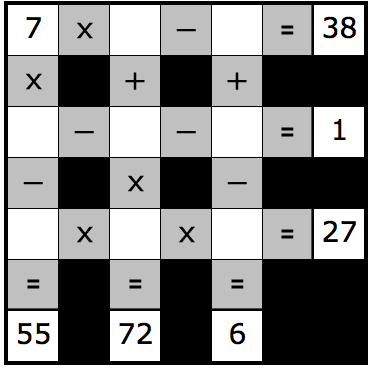
\includegraphics[scale=0.4]{exemplo_mathemagrids}
\end{center}

Neste exemplo, já é dada uma {\it{hint}}, o $7$ que aparece na primeira linha, primeira coluna.

\section{Z3}
\paragraph{} 
Como {\sc{SMT-solver}} estamos a usar o {\sc{z3}} Theorem Prover da Microsoft Research. Este, é usado em vários softwares de verificação formal. 
\\

Como linguagem de interface com o {\sc{z3}} preferimos usar o {\sc{python}} {\sc{z3Py}} devido à sua {\sc{API}} fácil de usar e devido a ser uma linguagem simples e eficaz para o que queriamos fazer.

\section{{\it{solveMathemaGrids.py}}}

\paragraph{} 
O $solveMathemaGrids.py$ é invocado como um ficheiro python qualquer:
\begin{verbatim}
 $ solveSurvo.py <ficheiro\_input>
\end{verbatim}
por exemplo,
\begin{verbatim}
 $ solveSurvo.py exemplo_1.txt
\end{verbatim}

Caso consiga resolver o puzzle, é imprimido no ecra o output, ou seja, o puzzle completo com os as soluções. É necessário que o {\sc{z3}} esteja instalado e conectado com o {\sc{python}}.

\subsection{Ficheiros input}

\paragraph{} 

Para representar um tabuleiro de {\sc{MathemaGrids}} (o do exemplo) usamos o seguinte ficheiro de texto:
\begin{center}
\begin{verbatim}
7*.-.=38
*,+,+
.-.-.=1
-,*,-
.*.*.=27
=,=,=,=
55,72,6
\end{verbatim}
\end{center}

Os $"."$ representam os espaços que têm que ser preenchidos com números e as $","$ representam os espaços que, apesar de existirem no tabuleiro, não podem ser inseridos com números. 
\\

Também estão representadas as operações sendo o {\bf{*}} a multiplicação, o  {\bf{+}} a soma, {\bf{-}} a subtração e {\bf{/}} a divisão. 

\subsection{Ficheiros output}
\paragraph{} 
O {\sc{MathemaGrids}} dá como output um ficheiro com a representação da matriz obtida e os valores que as linhas e as colunas que respeitam as operações dadas como imput.


O do exemplo :
\begin{center}
%\begin{verbatim}
{\bf{------> falta o output}}
%\end{verbatim}
\end{center}

\subsection{Codificação do {\sc{MathemaGrids}}}
\paragraph{} Para codificar o puzzle,usamos as seguintes propriedades (descritas em {\url{https://www.brainbashers.com/mathemagrids.asp}}):
 \begin{enumerate}
 \item Usar todos os digitos de 1 a $m*m$ (no nosso exemplo, até $9$);
 \item Nenhum número pode ser repetido;
 \item As operações são feitas da esquerda para a direita e de cima para baixo, sendo a ordem de prioridade normal da matemática ignorada;
 \item Não podem existir divisões por 1 nem multiplicações por 1;
\item Em nenhum ponto, os resultados intermédios do cálculo são valores infeiores a zero.
 \end{enumerate}

As variaveis $x$\_$membros$ e $y$\_$membros$ representam a quantidade de espaços em que o jogador pode inserir números nas linhas e nas colunas respetivamente. As regras usadas são:

 \begin{enumerate}
 \item 

\begin{verbatim}
[ And(1 <= X[j][i], X[j][i] <= x_membros*y_membros)
 for i in range(x_membros) for j in range(y_membros) ]
\end{verbatim}
 \item

\begin{verbatim}
[ Distinct([X[j][i] for i in range(x_membros)  
for j in range(y_membros)]) ]
\end{verbatim}

 \item Para garantir que as operações são feitas na ordem correta, escrevemos as equações horizontais e verticais que, neste exemplo são : \\
{\bf{------> faltam aqui as equações}}
\item 

\begin{verbatim}
div_mult_por_1 = []
for i in range(len(table)):
    for j in range(len(table[i])):
        if (table[i][j]=='/' or table[i][j]=='*' ):
            if (i%2==0):
                div_mult_por_1.append(Not(X[i/2][(j+1)/2] == 1))
            else:
                div_mult_por_1.append(Not(X[(i+1)/2][j/2] ==1))
\end{verbatim}

\item Como a operação critica para isto acontecer é apenas a subtração: 

\begin{verbatim}
bigger_than_zero = []
for i in range(len(table)):
    for j in range(len(table[i])):
        if (i%2==0):
            if(table[i][j]=='-'):
                bigger_than_zero.append(Not(X[i/2][((j+1)/2)-1] 
                - X[i/2][(j+1)/2] < 0))
                bigger_than_zero.append(Not(X[((i+1)/2-1)][j/2] 
                - X[((i+1)/2)][(j+1)/2] < 0))
\end{verbatim}


 \end{enumerate}

\end{document}